\icode{E-MI-SI-L2-261106-001}
如图所示，一物块置于水平地面上。当用与水平方向成\qty{60}{\degree}角的力\(F_1\)拉物块时，物块做匀速直线运动；当改用与水平方	向成\qty{30}{\degree}角的力\(F_2\)推物块时，物块仍做匀速直线运动。若\(F_1\)和\(F_2\)的大小相等，则物块与地面之间的动摩擦因数为\paren[]

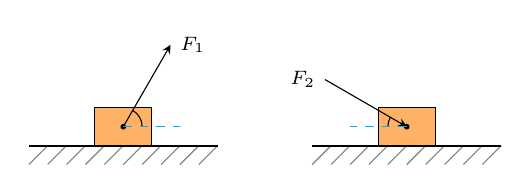
\begin{tikzpicture}[scale=1.2,>=stealth,font=\scriptsize]
	\begin{scope}
		\draw[fill=orange!60] (-.3,-.2) rectangle(.3,.2);
        \fill (0,0) circle(.03);
		\foreach \x in {-1,-.8,...,.8}
			\draw[gray] (\x,-.4)--++(.2,.2);
		\draw[thick] (-1,-.2)--(1,-.2);
		\draw[->] (0,0)--(60:1)node[right]{\(F_1\)};
        \draw (.2,0) arc(0:60:.2);
		\draw[dashed,cyan] (0,0)--(.6,0);
	\end{scope}
	\begin{scope}[xshift=3cm]
		\draw[fill=orange!60] (-.3,-.2) rectangle(.3,.2);
        \fill (0,0) circle(.03);
		\foreach \x in {-1,-.8,...,.8}
			\draw[gray] (\x,-.4)--++(.2,.2);
		\draw[thick] (-1,-.2)--(1,-.2);
		\draw[->] (150:1)node[left]{\(F_2\)}--(0,0);
		\draw (-.2,0) arc(180:150:.2);
		\draw[dashed,cyan] (0,0)--(-.6,0);
	\end{scope}
\end{tikzpicture}
\begin{choices}
	\item\(\sqrt{3} - 1\)
	\item\(2 - \sqrt{3}\)
	\item\(\dfrac{\sqrt{3} - 1}{2}\)
	\item\(\dfrac{2 - \sqrt{3}}{2}\)
\end{choices}
\begin{answer}
    B\qquad 提示：
\end{answer}